\documentclass{article}
\usepackage[spanish]{babel}
\usepackage[letterpaper,top=2cm,bottom=2cm,left=3cm,right=3cm,marginparwidth=1.75cm]{geometry}

\usepackage{amsmath}
\usepackage{graphicx}
\usepackage[colorlinks=true, allcolors=blue]{hyperref}
%---------------------------------------------------------
\begin{document}
\maketitle

\thispagestyle{empty}
\begin{center}
    \includegraphics[width=0.4\textwidth]{Universidad_Católica_de_Temuco_logo.jpg}
\end{center}
\vspace{2cm}

\begin{center}
    {\Huge \textbf{Laboratorio n°2: Introduccion a GitHUb y Latex}} \\[4cm]
    {\large \textbf{Nombre:}}\\[0.5cm] Franchesca Marcial\\[0.5cm]
    {\large \textbf{Profesor:}}\\[0.5cm] Guido Mellado \\[0.5cm]
    {\large \textbf{Ayudante:}}\\[0.5cm] Fernando Valdés \\[0.5cm]
\end{center}

\newpage
\renewcommand{\contentsname}{Índice}
\tableofcontents
\newpage
\section{Explicaciones}
\subsection{herencia,clase abstracta,polimorfismo,interfaz.}

\begin{itemize}
    \item herencia: La herencia es un tipo de relación entre tablas de entidad, donde existe la superclase y la clase hijo, donde la clase hijo 'hereda' todos los atributos y métodos de la superclase, pero aun as la clase hijo puede modificar y agregar nuevos atributos y métodos.

    
    \item clase abstracta: Se trata de una clase que no puede ser instanciada, eso quiere decir que no se pueden crear objetos directamente en ella, ya que más bien está diseñada para ser como clase plantilla para otras clases, como las @dataclass.
    
    \item polimorfismo: El polimorfismo es cuando tenemos una superclase y muchas clases hijos y todas las clases hijos heredan un método en común , por ejemplo método de hacer un ruido, en lugar de crear variables para cada tipo específico, usamos la clase base para referirnos a cualquier objeto que pertenezca a la jerarquía y el código solo llama a un solo método sin verificar el objeto que hace el ruido.
    
    \item interfaz: Es como un decorador, un contrato o un conjunto de reglas que una clase debe aceptar y cumplir, además, tampoco se pueden crear objetos directamente.
\end{itemize}





\section{Ejemplos en Python y diagramas.}

En esta sección se presentan ejemplos prácticos en lenguaje Python para ilustrar los conceptos de Herencia, Clases Abstractas, Polimorfismo e Interfaces. Cada ejemplo muestra cómo se aplican estos principios en la programación orientada a objetos (POO).

\subsection{Ejemplo de Herencia}
\thispagestyle{empty}
\begin{center}
    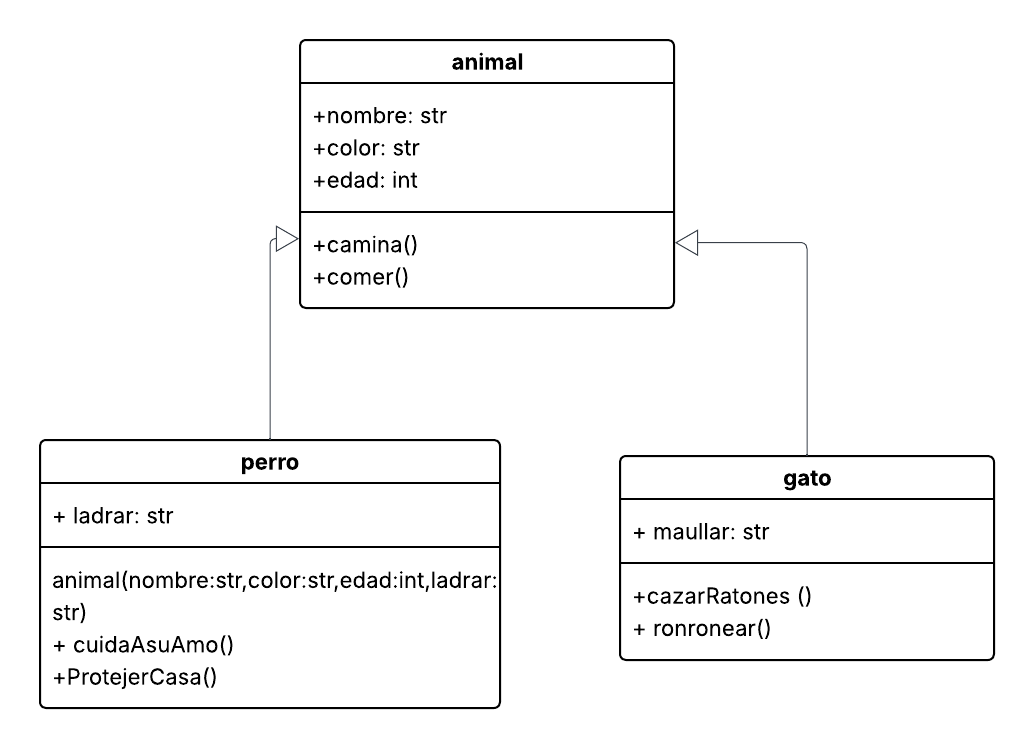
\includegraphics[width=0.5\textwidth]{Diagrama herencia.png}
\end{center}
\vspace{1cm}
En este diagrama de ejemplo la clase perro y la clase gato heredan todos los atributos y metodos de su clasepadre llamada "animal" y se puede ver que tambien cada clasehijo agrega su propio atributo y sus propios metedos.

\subsection{Ejemplo de clase abstract}
\thispagestyle{empty}
\begin{center}
    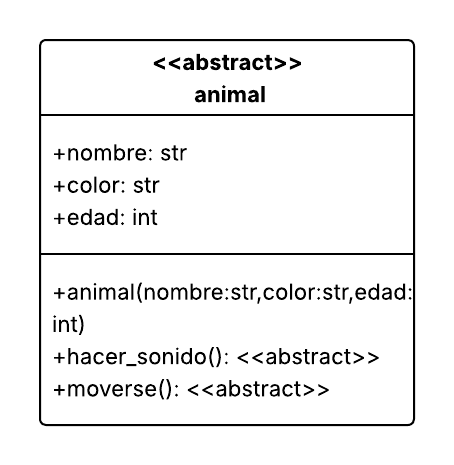
\includegraphics[width=0.4\textwidth]{clase abstract.png}
\end{center}
\begin{verbatim}
from abc import ABC, abstractmethod

class Animal(ABC):
    def __init__(self, nombre: str, color: str, edad: int):
        self.nombre = nombre
        self.color = color
        self.edad = edad

    @abstractmethod
    def hacer_sonido(self):
        pass

    @abstractmethod
    def moverse(self):
        pass
\end{verbatim}

Este ejemplo ilustra cómo definir métodos abstractos que las subclases deberán implementar, garantizando que todas compartan una estructura común pero con comportamientos específicos.


\subsection{Ejemplo de Polimorfismo}

\begin{verbatim}
class Gato(Animal):
    def hablar(self):
        return "Miau!"

animales = [Perro("Firulais"), Gato("Michi"), Animal("Desconocido")]

for a in animales:
    print(f"{a.nombre}: {a.hacer_sonido()}")
\end{verbatim}

El polimorfismo permite que diferentes objetos respondan de manera distinta al mismo método \texttt{hablar()}, sin necesidad de conocer su tipo específico.
\newpage
\subsection{Ejemplo de Interfaz}

\begin{verbatim}
from abc import ABC, abstractmethod

class Volador(ABC):
    @abstractmethod
    def volar(self):
        pass

class Pajaro(Volador):
    def volar(self):
        return "El pájaro está volando"

class Avion(Volador):
    def volar(self):
        return "El avión despega"

# Uso
objetos = [Pajaro(), Avion()]
for o in objetos:
    print(o.volar())
\end{verbatim}

En este caso, la clase \texttt{Volador} actúa como una interfaz: define un conjunto de métodos que las clases hijas deben implementar.


\section{Method Resolution Order (MRO)}

El \textbf{MRO (Method Resolution Order)} define el orden en que Python busca los métodos y atributos en una jerarquía de herencia múltiple.  
Esto es importante cuando una clase hereda de varias clases al mismo tiempo.

\subsection{Ejemplo de MRO}

\begin{verbatim}
class A:
    def saludo(self):
        print("Hola desde A")

class B(A):
    def saludo(self):
        print("Hola desde B")

class C(A):
    def saludo(self):
        print("Hola desde C")

class D(B, C):
    pass

d = D()
d.saludo()
print(D.mro())
\end{verbatim}

En este caso, Python imprimirá:

\begin{verbatim}
Hola desde B
[<class '__main__.D'>, <class '__main__.B'>, 
 <class '__main__.C'>, <class '__main__.A'>, <class 'object'>]
\end{verbatim}

El resultado muestra que el orden de búsqueda de métodos sigue la secuencia:  
\texttt{D → B → C → A → object}.  
Esto significa que Python ejecuta el método \texttt{saludo()} de la clase \texttt{B} primero, respetando el MRO.

\centering
\end{document}